\section{Preliminaries}
\label{sec:related}

In this section, we first summarize and review some related preliminary works of on-chip power grid EM-induced IR drop analysis and mitigation approaches.

\subsection{Full-chip EM-induced IR drop analysis}
\label{subsec:emspice}
As mentioned in the previous section, EM is a physical phenomenon that can lead to resistance increase or even open-wire segments.  The IR drop of the power grid wires may change due to the EM-induced aging effect. This means we have to consider the power girds IR drop as time-varying characters~\cite{SunYu:TDMR'20, Huang:TCAD'15, Chatterjee:2018TCAD,SukharevNajm:2018TDMR}. 
On the other hand, the failed wire segments change the current distributions of all the interconnect wires, which may further accelerate the failure process. Hence, to emulate the on-chip power grid IR-drop after the aging effect, one has to consider the interplay between the two physics: electrical characteristics and hydrostatic stress in the interconnect wires.

{\it EMspice}~\cite{SunYu:TDMR'20,EMspiceSourceCode} is an open source tool that conducts the full-chip power grid network coupled EM-IR drop simulation with the dynamic interplay between the hydrostatic stress and electronic current/voltage. It solves the coupled time-varying partial differential equations in the time domain to obtain the stress evolution, and finally reports resulted IR drop and EM failure hotspots at the target aging time, such as 10 years.  The tool consists of a finite difference time domain (FDTD) solver for EM stress and a linear network DC solver for IR drop. The linear network IR drop solver passes time-dependent current densities and P/G layout information to the finite difference time domain FDTD EM solver, and the FDTD EM solver provides the IR drop solver with new resistance information. These two simulations are coupled together and must be solved together, which can be described as

%\begin{align}
%	\label{eq:em}
%		&{\bf C} \dot{\sigma}(t)  = {\bf A} \sigma(t) + {\bf P}I(t),  \\
%		&\mathcal{V}_v(t)  = \int_{\Omega_L}\frac{\sigma(t)}{B}d\mathcal{V},  \\ 
%		&{\bf M}(t) \times u(t)  = {\bf P} I(t), \\
%		&{\bf \sigma}(0)  = [\sigma_1(0), \sigma_2(0), ..., \sigma_n(0)] \,\, ,at \,\, t = 0 
%\end{align}

\begin{align}
	\label{eq:em}
	\begin{split}
		&{\bf C} \dot{\sigma}(t)  = {\bf A} \sigma(t) + {\bf P}I(t),  \\
		&\mathcal{V}_v(t)  = \int_{\Omega_L}\frac{\sigma(t)}{B}d\mathcal{V},  \\ 
		&{\bf M}(t) \times u(t)  = {\bf P} I(t), \\
		&{\bf \sigma}(0)  = [\sigma_1(0), \sigma_2(0), ..., \sigma_n(0)] \,\, ,at \,\, t = 0 
	\end{split}
\end{align}
In the above equations, ${\bf M}(t)$ is the time-varying power grid conductance matrix, as the resistance changes due to the EM failure process. ${{\bf P}}$ is the input matrix, and I(t) represents the current sources from the chip. ${{\bf C}}$ is the identity matrix, and ${{\bf A}}$ is the coefficient matrix. $\sigma_{n}(0)$ denotes the initial stress at time step $t = 0$, for node $n$. Thee stress from the previous simulation step is used as the initial condition for each new time step. Such iterative coupled analysis on a long target lifetime can be extremely time-consuming for large power grid networks.

There are some research efforts to facilitate the IR drop/EM-aware IR drop analysis by leveraging machine learning-based approaches to build the surrogate models, including ~\cite{LinFang:2018vts,Fang:2018dynireco,HoKahng:ICCAD'19,Xie:2020powernet,Sachin:ASPDAC'21} to reduce the evaluation time during the physical design process.  Lin {\it et al.}~\cite{LinFang:2018vts} tried to extract power and physical features from cells and layouts to conduct the full-chip dynamic IR drop analysis. Fang {\it et al.}~\cite{Fang:2018dynireco} proposed to train the models for the localized layout region to improve the scalability.  A convolutional neural network (CNN) model which incorporates design-dependent features during pre-processing was proposed by Xie {\it et al.}~\cite{Xie:2020powernet}. Ho {\it et al.}~\cite{HoKahng:ICCAD'19} presented incremental IR drop prediction and mitigation by applying more electrical and physical features to train the gradient-boosting framework. Chhabria {\it et al.}~\cite{Sachin:ASPDAC'21} proposed {\it IREDGe}, a CNN-based generative network method to predict on-chip IR drop contours with image-to-image and sequence-to-sequence translation tasks.
Recently Zhou {\it et al.} \cite{ZhouJin:ICCAD'20} considered more accurate physics-based EM effects into IR drop to build such surrogate models. It adopted the GAN-based structure to model the resulting EM-aware IR drops.  This method regards the time, 2D power grid structure with input current and voltages as input images (series of images) and outputs the voltage map images. Such a surrogate model can help speed up wire sizing by fast EM-aware IR drop estimation and the sensitivity of objective functions concerning the wire geometries. It was initially applied to localized PDN optimization and then has been extended to full-chip optimization~\cite{HanLiu:TCAD'22-23}.
However, the GAN-based models suffer from the difficulties of training the generator and discriminator together. Also, the GAN model's deterministic latent variable encoding and decoding approach make the latent space lack of continuity and interpretability and less generative capability (due to non-regulated latent space), eventually affecting the prediction accuracy.


\subsection{Existing EM-aware PDN optimization}
 \label{subsec:exist_pgfix}
Besides the full-chip aging-aware IR-drop estimation, one also needs to fix or alleviate the excessive IR-drop to ensure a robust PDN design. Lots of past research applies nonlinear methods~\cite{ChBr:TCAD'88,DuMa:DAC'89,Tan:DAC'99,Wang:TCAD'05,ZhouSun:TVLSI'19, Sukharev:2019pg} to size the PDN wires properly. These optimization strategies aim to meet the IR drop requirement at the target lifetime or extend the main time to failure (MTTF) with minimized metal routing area.

The SLP-based method was proposed first in~\cite{Tan:DAC'99} based on Black's equation. Then this method was extended to consider multi-segment wires~\cite{ZhouSun:ASPDAC'18}. But this method can be too conservative as it requires all the wires to be immortal after optimization. Although, this method has been extended to consider a targeted lifetime by allowing some wires to fail and optimizing the rest of the wires~\cite{ZhouSun:TVLSI'19}.  Recently~\cite{Sukharev:2019pg} proposed to directly optimize EM-induced IR drops on the time-varying power grid networks EM caused by EM-induced aging using the SLP method. However, the EM-induced IR drop is still computed by solving Korhonen equations, and the sensitivities of the IR drop with respect to the wires are calculated through the matrix-solving method.  
The solving process is severely time-consuming, especially when the power grid is enormous.


\subsection{Variational Autoencoder}
\label{subsec:vae_intro}
this paper adopts VAE~\cite{Diederik:arxiv'22} as the machine learning model for the EM-aware IR drop estimations. 
VAE follows a similar structure to autoencoder(AE).

As shown in Fig.\ref{fig:ae}, the traditional AE structure includes encoder and decoder structures. Input will be encoded to low-dimensional latent variables by the encoder and then decoded to the output by the decoder.  
The GAN model adopts the standard AE as a \textit{generator} to generate the result and uses an additional binary output CNN as the discriminative network only in the training stage to better train the autoencoder. 


\begin{figure}[htp]
	\centering
	\subfigure[]{
		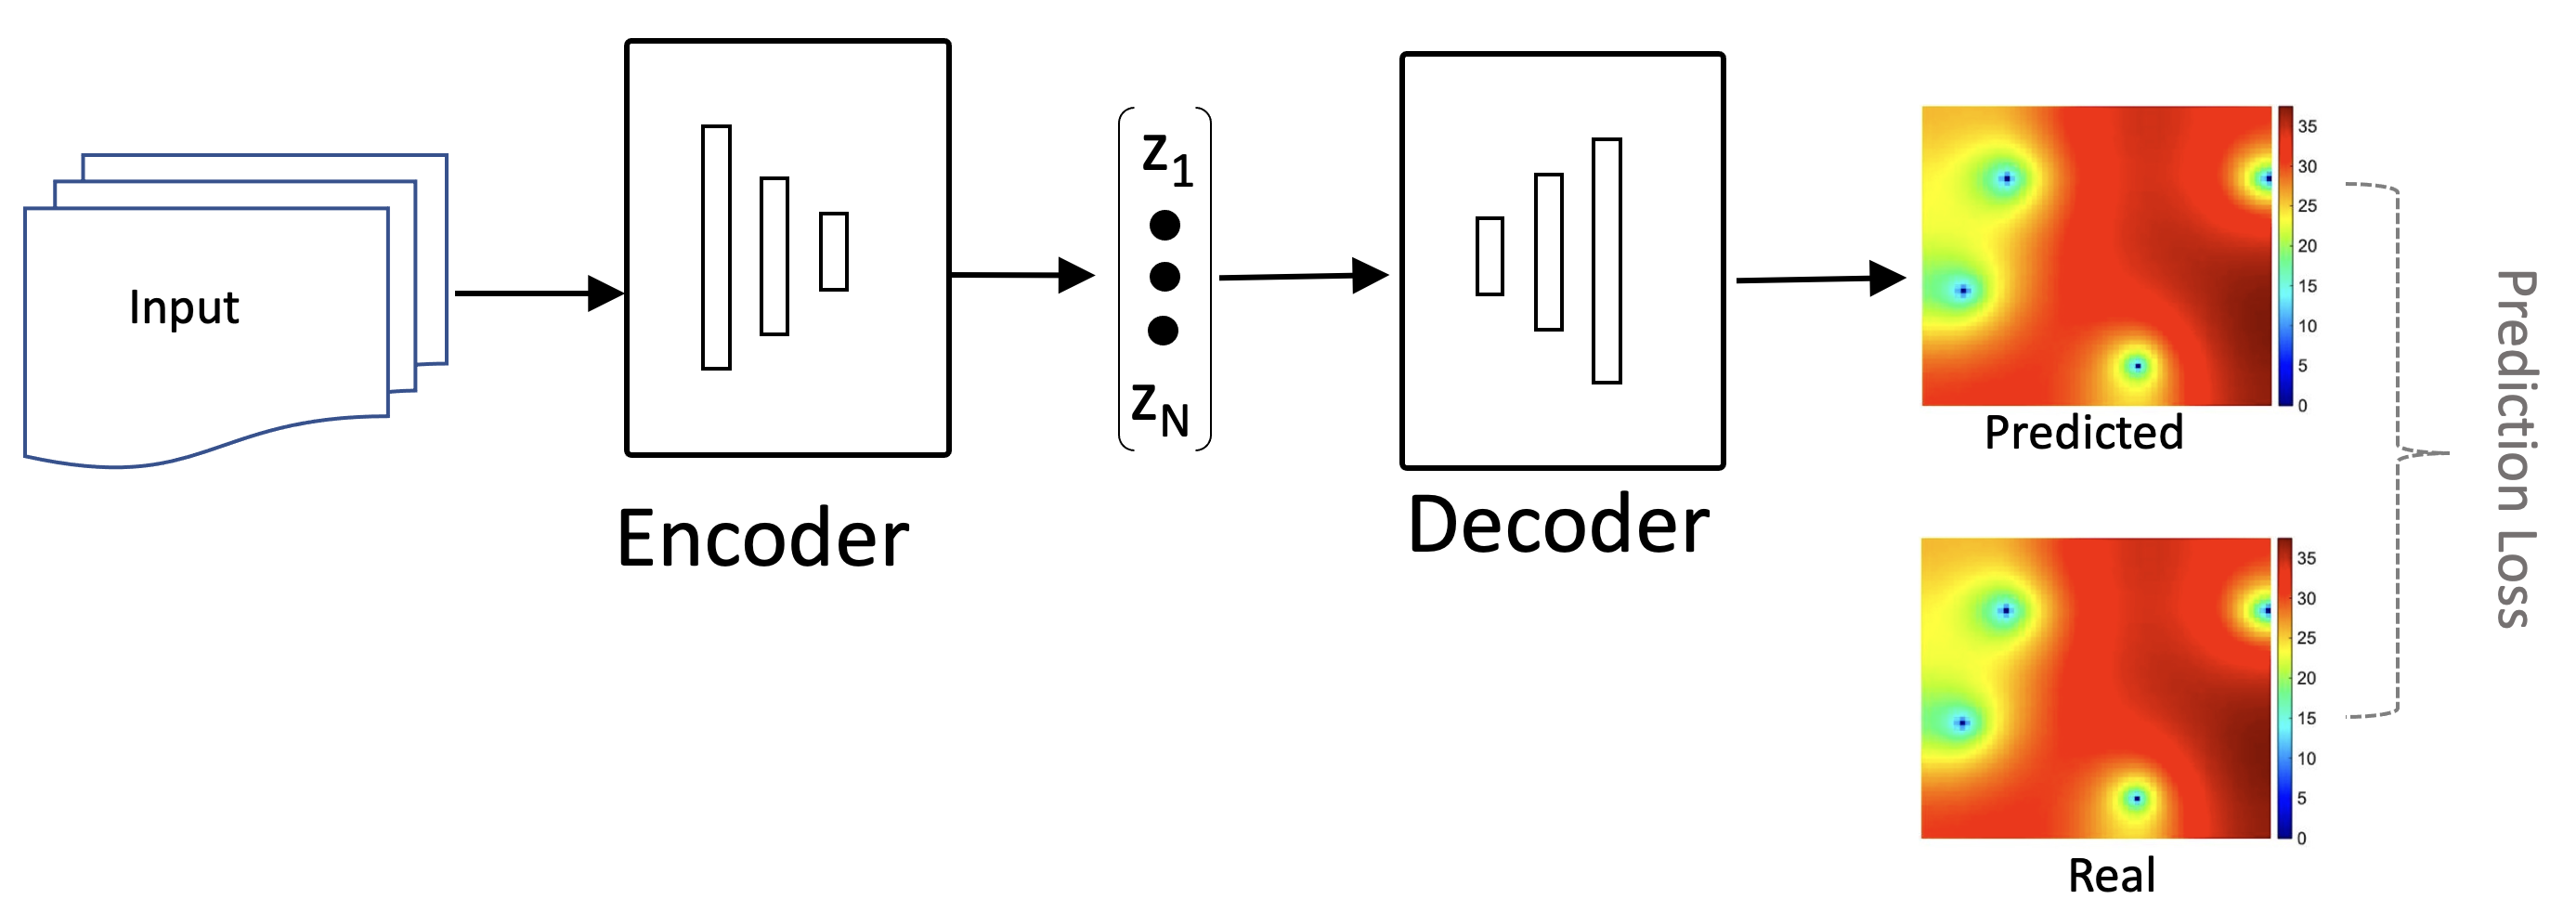
\includegraphics[width=0.9\columnwidth, height = 3cm]{./figs/ae_brief.eps}
		\label{fig:ae}}
	\subfigure[]{
		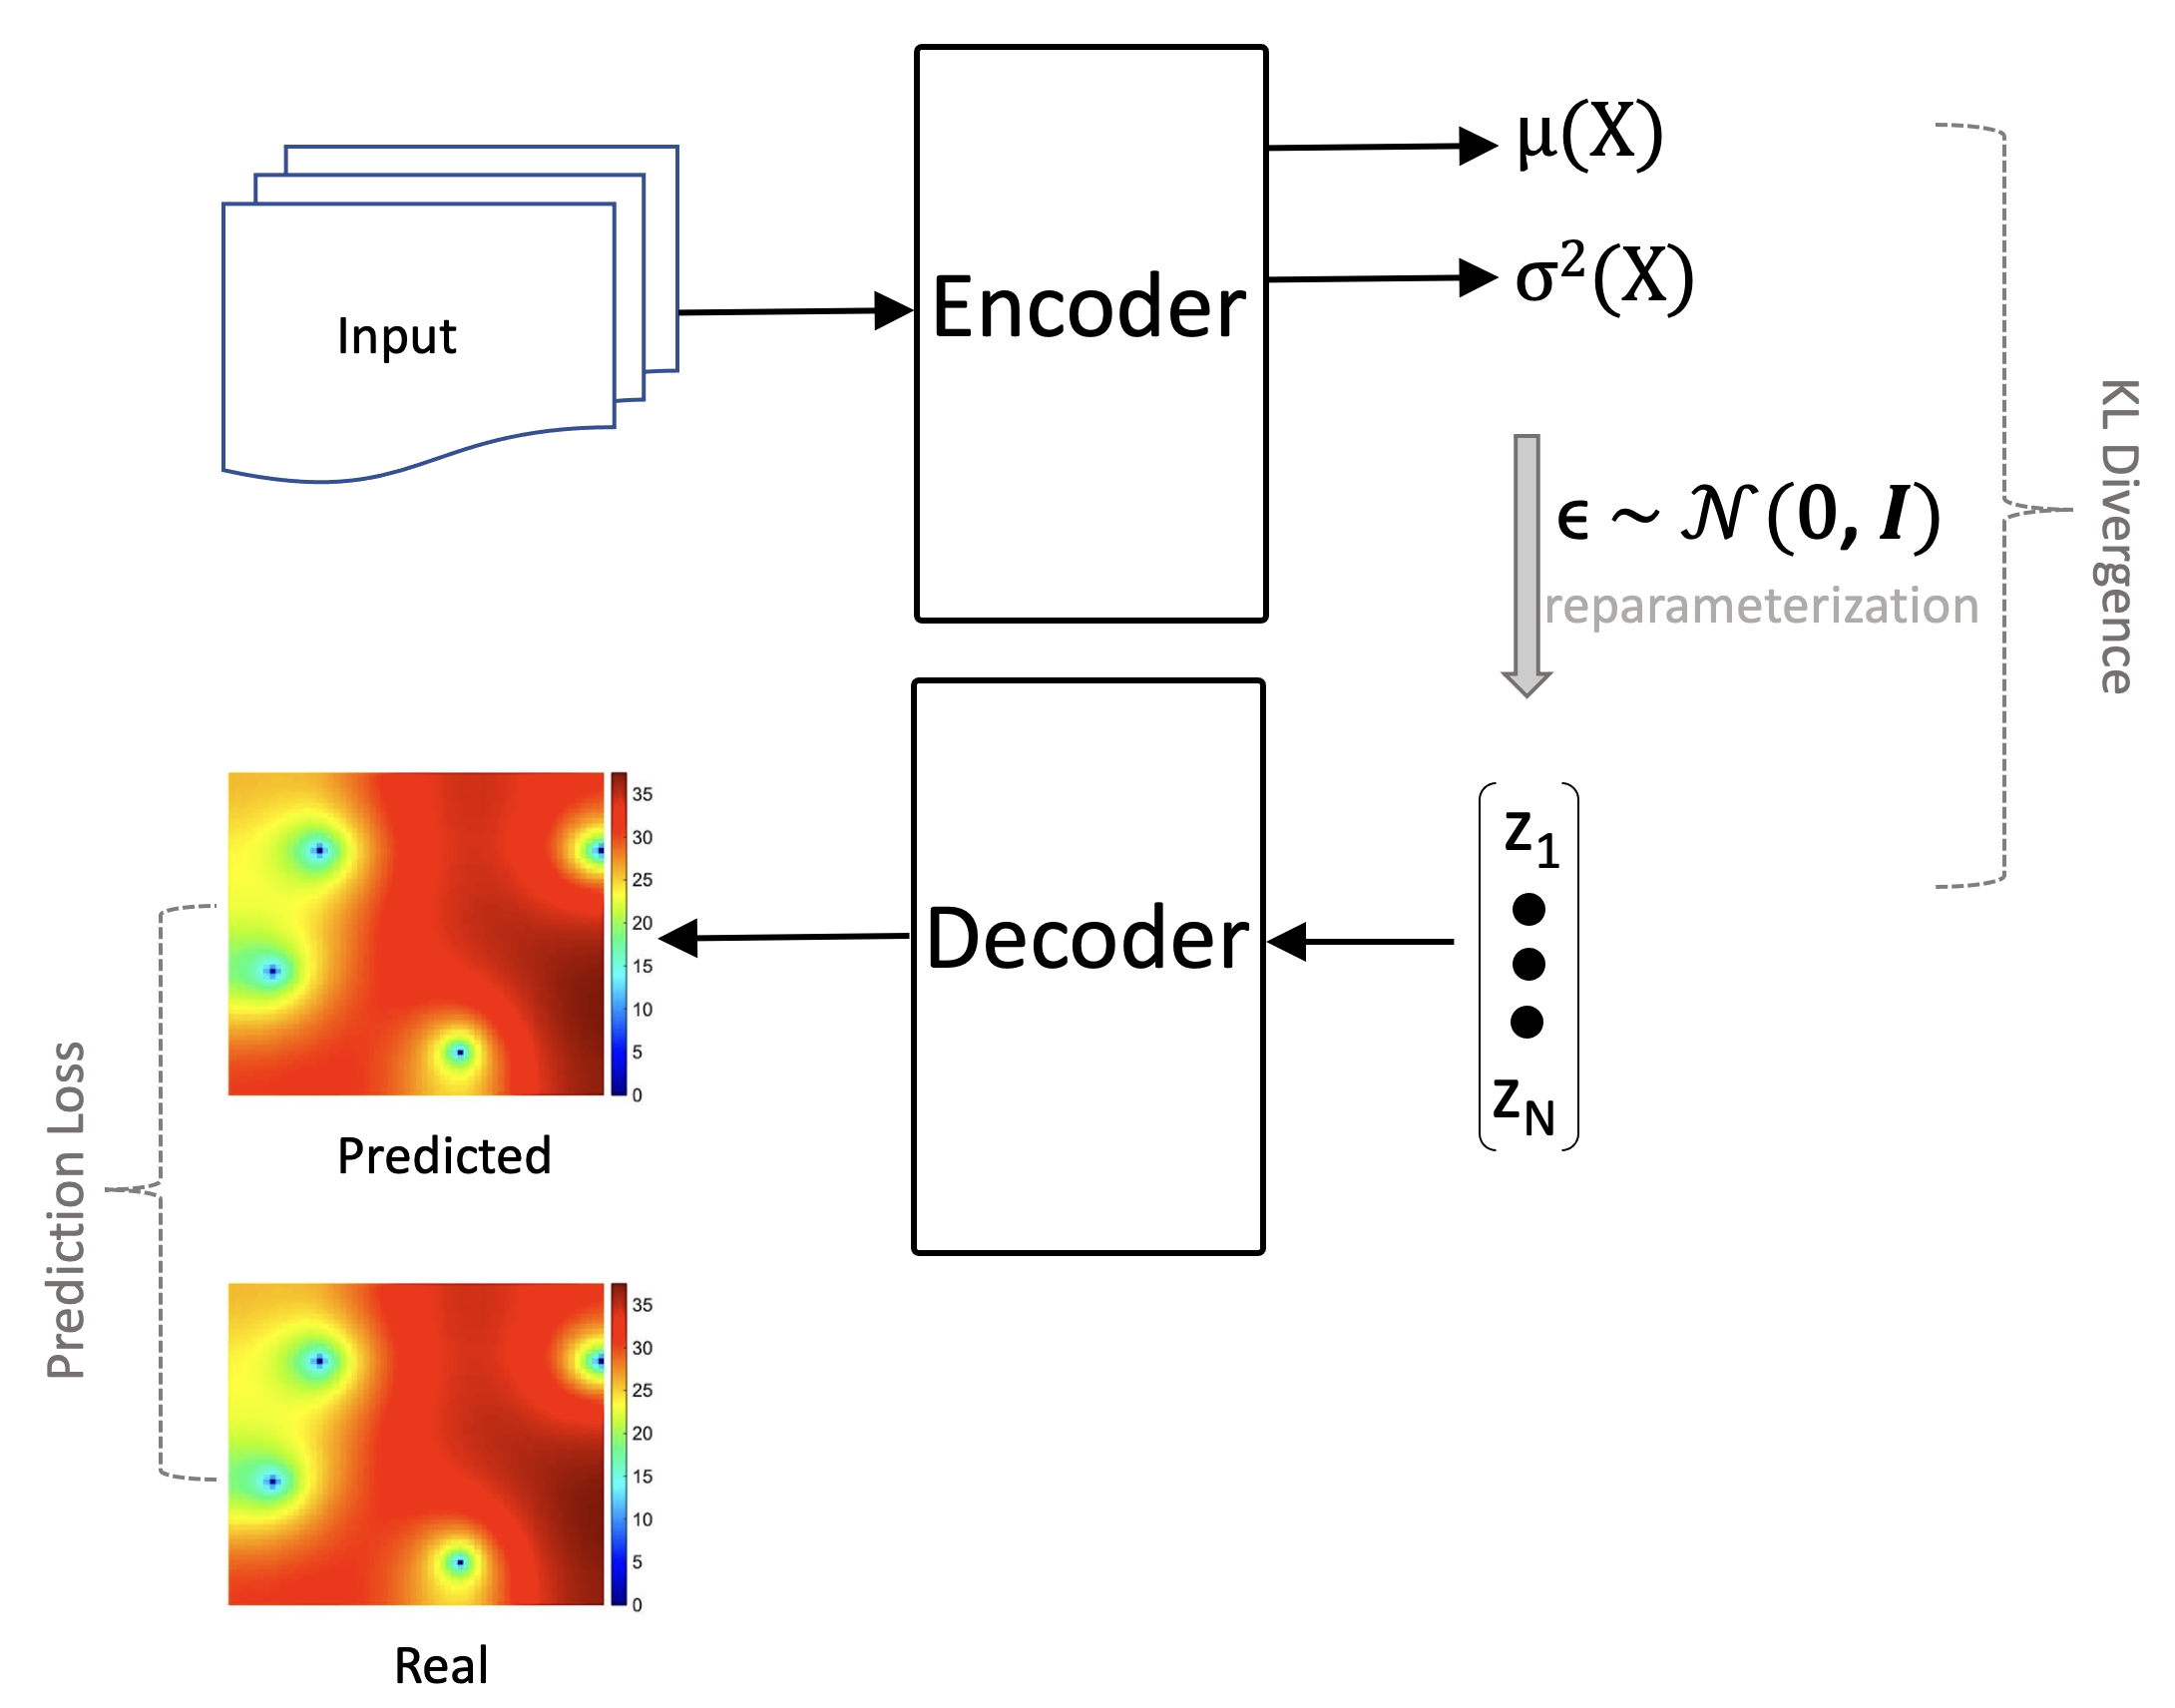
\includegraphics[width=0.8\columnwidth]{./figs/vae_brief.eps}
		\label{fig:vae}}
	\caption{(a) Architecture of an auto encoder (b)Architecture of a variational auto encoder }
	\label{fig:compare_ae_vae}
\end{figure}


 
Variational autoencoder, as shown in  Fig.\ref{fig:vae}, is a unique generative model derived from the standard autoencoder, which is used to generate new data similar to the input data it's trained on. 
Compared to the traditional autoencoder structure, VAE does not directly encode the input to a determined latent variable. Instead, it is encoded to a distribution over the latent space $Q(Z|X)$, and then sampled from this distribution to generate a latent variable for the decoder. This step is crucial to the VAE's characteristics over AE and AE-based GAN models, such as latent space  interpretability, and training stability.
Interpretability of latent space means that the latent space is smooth and interpretable, enabling friendly properties like the ability to interpolate between different points in the latent space and generate new samples that exhibit a smooth transition between the characteristics of the original points. On the other hand, AE does not explicitly enforce such a structure, making the latent space less interpretable and interpolations might not always produce meaningful outputs. 
Usually, the VAE latent variable $z$ is generated using a reparameterization approach to ensure the model backpropagation with gradient descent. We denote the mean of $Q(Z|X)$ as $\mu$ and the standard deviation as $\sigma$, and sample $\epsilon \sim \mathcal{N}(\textbf{0}, \textbf{I} ) $, then compute z as equation.\eqref{eq:z_compute}:

\begin{equation}
	\label{eq:z_compute}
	z = \mu(\textit{X}) + \sigma \ast \epsilon(\textit{X})
\end{equation}








